\documentclass{article}
\usepackage{graphicx}
\usepackage{amsmath}
\usepackage[brazilian]{babel}
\usepackage{amsthm}
\usepackage{hyperref}
\usepackage{xcolor}

\renewcommand{\refname}{Referências}

\theoremstyle{definition}
\newtheorem{definition}{Definição}[section]

% Custom commmands
\newcommand\norm[1]{\left\lVert#1\right\rVert}

\def \quantity#1#2#3{\vec{#1}_{#2}^{#3}}
\def \quantitysc#1#2#3{{#1}_{#2}^{#3}}
\def \quantityg#1#2#3#4#5{\vec{#1}_{#2, #3}^{#4, #5}}
\def \quantitygsc#1#2#3#4#5{{#1}_{#2, #3}^{#4, #5}}
\def \pos#1#2{\quantity{r}{#1}{#2}}
\def \desloc#1#2{\quantity{d}{#1}{#2}}
\def \deslocsc#1#2{\quantitysc{d}{#1}{#2}}
\def \deslocg#1#2#3#4{\quantityg{d}{#1}{#2}{#3}{#4}}
\def \deslocgsc#1#2#3#4{\quantitygsc{d}{#1}{#2}{#3}{#4}}

\title{Simulação da Reologia e dos Padrões de Movimento de Tecidos Celulares com Anéis Ativos}
\author{Marcos Pasa e Leonardo Brunnet}

\begin{document}

\maketitle

\section{Introdução}
\begin{figure}[h]
    \centering
    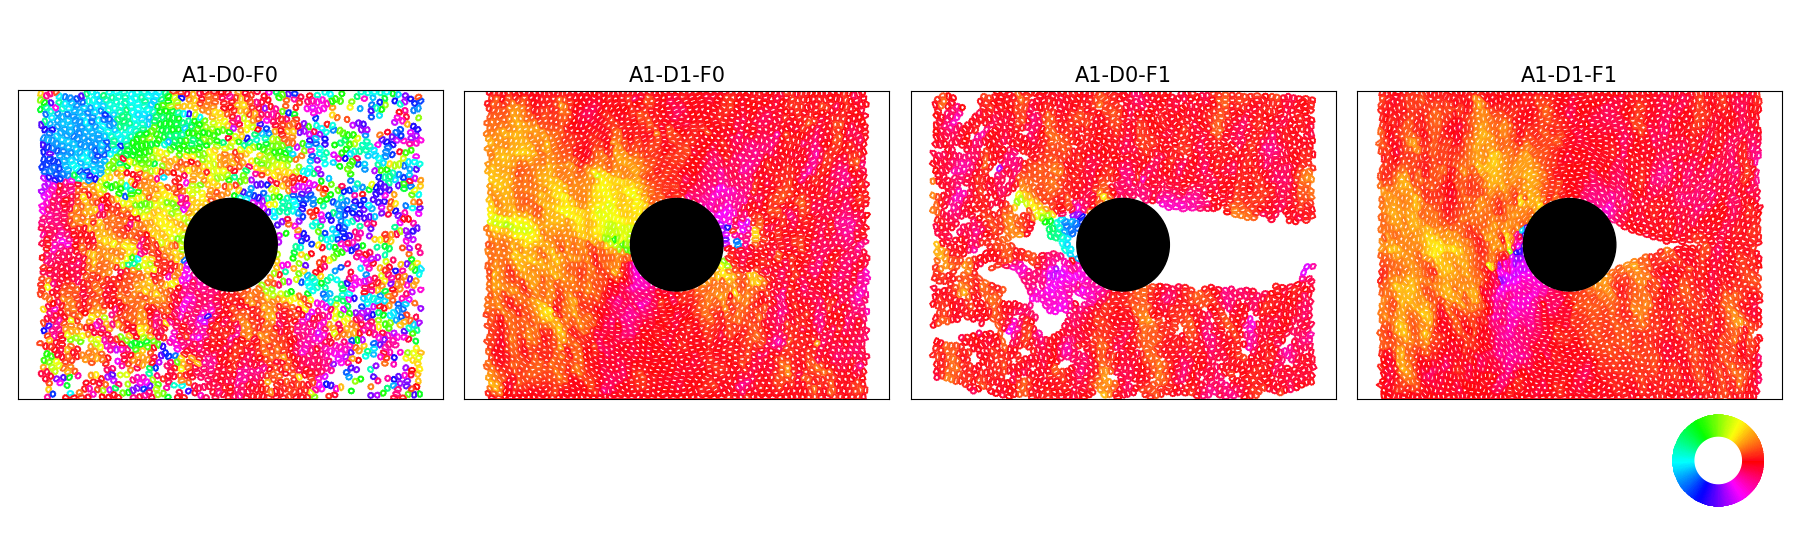
\includegraphics[width=\textwidth]{figuras/high_align_vel_color.png}
    \caption{Teste}
    \label{}
\end{figure}

Cicatrização de feridas, morfogênese e evolução tumoral são processos essenciais nos organismos vivos e motivam a pesquisa de fenômenos relacionados à organização multicelular. Em particular é importante entender características físicas tais como viscosidade, plasticidade e elasticidade associadas a trocas de posições das células. Embora a genética subjacente determine as mudanças das interações microscópicas, ao final serão as características físicas que estarão em jogo na organização. Defeitos topológicos associados à ordem nemática, invaginações devido a contrações do cortex de membranas sendo  exemplos característicos. Modelos computacionais de sistemas multicelulares são ferramentas robustas para testar hipóteses e ganhar conhecimento sobre tais sistemas.

Diversos modelos de células ativas já foram desenvolvidos, os mais simples tem como grau de liberdade o centro da célula, nesse caso as células podem ser representadas como esferas com volume de exclusão ou polígonos de uma tesselação de Voroni. A principal vantagem desses modelos é sua simplicidade e desempenho computacional, porém eles não são adequados para modelar situações mais complexas. Sofisticando um pouco mais, existem os modelos em que o grau de liberdade é o contorno da célula, em que as células podem ser descritas por pixels semelhantes a imagens experimentais (modelo celular de Potts), vértices de um polígono livre para se mover e interagir par a par, e até como um campo de fases contínuo.
\textcolor{red}{Aqui tem de colocar referências para os diferentes modelos mencionados.}

Dessa forma, o presente trabalho tem por objetivo implementar e explorar um modelo teórico-computacional para células biológicas com grau de liberdade no contorno das mesmas. Foi escolhido o modelo apresentado por Teixeira \textit{et al}.(\cite{teixeira_single_2021}, \cite{teixeira_segregation_2024}), em que células são representadas por polígonos cujos vértices são partículas ativas com volume de exclusão e mecanismo de auto-alinhamento. As partículas são conectadas por molas, assim possibilitando a deformação do formato das células.

Para estudar o modelo, escolhemos simular um fluxo de células confinado em um corredor com um obstáculo circular no centro (fluxo de Stokes). 
Seguimos no mesmo espirito no trabalho feito por Beatrici \textit{et al}. \cite{beatrici_comparing_2023}, em que 5 modelos de células móveis foram comparados.


A matéria ativa é uma área de pesquisa em física que tem ganhado destaque nas últimas décadas. Ela se concentra em sistemas fora do equilíbrio que exibem comportamentos coletivos surpreendentes devido à atividade intrínseca de suas partículas. Neste projeto de pesquisa, exploraremos o comportamento do modelo teórico-computacional de células biológicas proposto por Teixeira \textit{et al}.(\cite{teixeira_single_2021}, \cite{teixeira_segregation_2024})



\section{Objetivos}

\section{Modelo}
O modelo de dinâmica molecular utilizado é inspirado nos trabalhos de Teixeira \cite{teixeira_single_2021}, \cite{teixeira_segregation_2024} e nesta seção vamos apresentá-lo. Células são modeladas por estruturas chamadas de anéis ativos. Um anel ativo é composto por uma cadeia de partículas ativas, com mecanismo de auto-alinhamento e exclusão de volume, conectadas por molas. Primeiramente serão apresentadas as energias envolvidas, em sequência as forças provenientes dessas energias e por fim as equações de movimento.

\subsection{Energias}
Considere um sistema de $N$ anéis ativos compostos de $n$ partículas cada um. Vamos definir as seguintes quantidades:

\begin{itemize}
    \item $\pos{i}{\nu}$: posição da i-ésima partícula do $\nu$-ésimo anel.
    \item $\desloc{i}{\nu} := \pos{i}{\nu} - \pos{i-i}{\nu}$: Deslocamento entre partículas vizinhas do mesmo anel.
    \item $\quantityg{d}{i}{j}{\nu}{\sigma} := \pos{i}{\nu} - \pos{j}{\sigma}$: Deslocamento entre a partícula $i$ no anel $\nu$ e a partícula $j$ no anel $\sigma$.
\end{itemize}
Daqui em diante, fica subtendido que os índices possuem bordas periódicas, ou seja, os índices $(n+1)$ e $1$ se referem a mesma partícula, assim como os índices $-1$ e $n$.

A energia potencial proveniente da mola que conecta as as partículas ($i-1$) e $i$ no anel $\nu$ é

\begin{equation}
    {\{U_m\}}_{i}^{\nu} = \frac{k_m}{2}(\deslocsc{i}{\nu} - l_0)^2
\label{eq:spring_pot}
\end{equation}
em que $k_m$ é a constante da mola e $l_0$ seu comprimento de equilíbrio.

A próxima energia dá origem a uma força que tende a preservar a área dos anéis, para escrevê-la precisamos da área do anel $\nu$, que pode ser calculada com a seguinte expressão \footnote{O módulo da expressão da área (eq. [\ref{eq:ring_area}]) pode ser retirado contanto que a iteração das partículas seja feita no sentido anti-horário.}

\begin{equation}
    A_\nu = \frac{1}{2}\bigg|\sum_{i=1}^{n}\pos{i}{\nu} \times \pos{i+1}{\nu} \bigg| 
\label{eq:ring_area}
\end{equation}
portanto, a energia potencial associada a força que tende a preservar a área do anel $\nu$ é

\begin{equation}
    {\{U_A\}}_{\nu} = \frac{k_a}{2}(A_{\nu} - A_0)^2
\label{eq:area_pot}
\end{equation}
em que $k_a$ é um parâmetro que controla a intensidade do potencial e $A_0$ é a área de equilíbrio.  $A_0$ controla a rigidez do anel, então caso seja de interesse mudar o tamanho do anel, por exemplo, alterar $l_0$ ou o número de partículas, mas mantendo a rigidez fixa, também é necessário alterar $A_0$. Uma forma de tornar o ajuste desse parâmetro mais conveniente é definir o parâmetro auxiliar $p_0$ (eq. [\ref{eq:p0}])

\begin{equation}
    p_0 := \frac{P}{\sqrt{A_0}} = \frac{n l_0}{\sqrt{A_0}}
    \label{eq:p0}
\end{equation}
em que $P = n l_0$ é o perímetro dos anéis. Todos os anéis com o mesmo valor de $p_0$, independente do seu tamanho, vão possuir a mesma rigidez.

Por fim, existe uma energia potencial associada a interação entre a partícula $i$ do anel $\nu$ com a partícula $j$ do anel $\sigma$. Esse potencial apenas depende da distância entre as partículas ($\deslocgsc{i}{j}{\nu}{\sigma}$) e tem um papel semelhante a um potencial Lennard-Jones: possui uma região de repulsão quando $\deslocgsc{i}{j}{\nu}{\sigma}$ é menor do que a distância de equilíbrio ($r_0$), e uma região de adesão quando $r_0 < \deslocgsc{i}{j}{\nu}{\sigma} < r_0 + b$, onde $b$ é o comprimento da região de adesão. $r_o$ acaba sendo o diâmetro efetivo das partículas. Tal potencial é descrito pela equação, %[\ref{eq:particle_particle_pot}]

\begin{equation}
\begin{aligned}
{\{U_p\}}_{i, i-1}^{\nu, \nu} &= {\{U_p\}}_{i, i}^{\nu, \nu} = {\{U_p\}}_{i, i+1}^{\nu, \nu} = 0, ~\forall~i, \nu \\
{\{U_p\}}_{i, j}^{\nu, \sigma} &= \begin{cases}
    \frac{k_{rep}}{2r_0}(\deslocgsc{i}{j}{\nu}{\sigma} - r_0)^2 &, 0 \leq \deslocgsc{i}{j}{\nu}{\sigma} \leq r_0 \\
    \frac{k_{atr}}{2b}(\deslocgsc{i}{j}{\nu}{\sigma} - r_0)^2 &, r_0 < \deslocgsc{i}{j}{\nu}{\sigma} < r_0 + b \text{ e } \nu \neq \sigma \\
    0 &, r_0 < \deslocgsc{i}{j}{\nu}{\sigma} < r_0 + b \text{ e } \nu = \sigma \\
    0 &, \deslocgsc{i}{j}{\nu}{\sigma} \geq r_0 + b 
\end{cases}
\end{aligned}
\label{eq:particle_particle_pot}
\end{equation}
onde $k_{rep}$ e $k_{atr}$ controlam a intensidade das forças de repulsão e adesão, respectivamente. Note que partículas vizinhas em um mesmo anel não contribuem para esse potencial, ou seja, elas apenas interagem através da mola que as conecta. Ainda, partículas no mesmo anel (que não são vizinhas) apenas podem se repelir. 

A energia potencial total do sistema ($U$) pode ser escrita da seguinte forma
\begin{equation}
\begin{aligned}
    U_m &= \sum_{\nu=1}^N\sum_{i=1}^{n} {\{U_m\}}_i^\nu \\
    U_A &= \sum_{\nu=1}^N {\{U_A\}}_\nu \\
    U_p &= \sum_{\nu < \sigma}^N \sum_{i, j}^n {\{U_p\}}_{i, j}^{\nu,   \sigma}  + \sum_{\nu=1}^N\sum_{i < j}^n {\{U_p\}}_{i, j}^{\nu, \nu}\\
    U & = U_m + U_A + U_p
\end{aligned}
\label{eq:total_energy}
\end{equation}

\subsection{Forças}
Estando definidas as expressões das energias, podemos derivá-las para obter as forças.

\subsubsection{Partículas vizinhas}
A força exercida na partícula $i$ no anel $\nu$ pelas suas vizinhas imediatas é
\begin{equation}
\begin{aligned}
    \quantity{\{F_m\}}{i}{\nu} &= -\quantitysc{\nabla}{i}{\nu}U_m = -\quantitysc{\nabla}{i}{\nu}\bigg[\quantitysc{\{U_m\}}{i}{\nu} + \quantitysc{\{U_m\}}{i+1}{\nu} \bigg] = \\ 
    &= -k_m (\deslocsc{i}{\nu} -l_0)\frac{\desloc{i}{\nu}}{\deslocsc{i}{\nu}} + k_m (\deslocsc{i+1}{\nu} -l_0)\frac{\desloc{i+1}{\nu}}{\deslocsc{i+1}{\nu}}
\end{aligned}
\label{eq:force_spring}
\end{equation}

\subsubsection{Partícula-Partícula}
É conveniente definir uma função indicadora de vizinhos em um anel, que chamaremos de $CN$. Dado a partícula $i$ no anel $\nu$ e a partícula $j$ no anel $\sigma$,  $CN_{i, j}^{\nu, \sigma}$ é 1 se as partículas pertencem ao mesmo anel ($\sigma = \nu$) e são vizinhas ($|i - j| \leq 1$). Uma forma de definir $CN$ é a seguinte
\begin{equation}
    CN_{i, j}^{\nu, \sigma} = \begin{cases}
        1,& \nu = \sigma \text{ e } |i - j| - \max\{0,  2(|i-j| - \lceil \frac{n}{2} \rceil) + n\bmod2 \} \leq 1 \\
        0,& \text{caso contrário}
    \end{cases}
\label{eq:close_neihbors}
\end{equation}
outra possível forma é \footnote{A igualdade $j=i\pm 1$ é verdadeira se ambos os índices se referem a mesma partícula, por exemplo, n = -1 avalia para verdadeiro.}
\[
CN_{i, j}^{\nu, \sigma} = \begin{cases}
        1,& (\nu = \sigma) \text{ e } (j=i \text{ ou } j = i \pm 1) \\
        0,& \text{caso contrário}
    \end{cases}
\]
Repare que a própria partícula é considerada como sua vizinha. Agora considere o conjunto de índices de partículas que estão a uma distância menor ou igual a $r_0$ em relação a partícula $i$ no anel $\nu$, e que não são vizinhas de $i$ 
\[
B_{rep} := \{(j, \sigma)~|~ \deslocgsc{i}{j}{\nu}{\sigma} \leq r_0 \text{ e } CN_{i, j}^{\nu, \sigma} = 0 \}
\]
também considere o conjunto de índices de partículas em diferentes anéis, que estão a uma distância maior do que $r_0$ e menor do que $r_0 + b$ em relação a partícula $i$ no anel $\nu$
\[
B_{adh} := \{(j, \sigma)~|~ r_0 < \deslocgsc{i}{j}{\nu}{\sigma} < r_0+b \text{ e } \nu \neq \sigma\}
\]
então a força de interação entre partícula-partícula atuando na partícula $(i, \nu)$ pode ser escrita como

\begin{equation}
\begin{aligned}
    \quantity{\{F_p\}}{i}{\nu} = &- \quantitysc{\nabla}{i}{\nu} U_p = \\ 
    = &-\sum_{(j, \sigma) \in B_{rep}} \frac{k_{rep}}{r_0}(\deslocgsc{i}{j}{\nu}{\sigma} - r_0)\frac{\deslocg{i}{j}{\nu}{\sigma}}{\deslocgsc{i}{j}{\nu}{\sigma}} ~~-\\
    &-\sum_{(j, \sigma) \in B_{adh}} \frac{k_{adh}}{b}(\deslocgsc{i}{j}{\nu}{\sigma} - r_0)\frac{\deslocg{i}{j}{\nu}{\sigma}}{\deslocgsc{i}{j}{\nu}{\sigma}}
\end{aligned}
\label{eq:force_particle_particle}
\end{equation}

\subsubsection{Preservação da área}
A força que preserva a área do anel $\nu$ atuando na partícula $i$ é

\[    
\quantity{\{F_A\}}{i}{\nu} = - \quantitysc{\nabla}{i}{\nu}U_A = -\quantitysc{\nabla}{i}{\nu} \{U_A\}_\nu
\]
desenvolvendo o gradiente, concluímos que a força é
\begin{equation}
    \quantity{\{F_A\}}{i}{\nu} = k_a (A_\nu - A_0) R_{\pi/2}\frac{\big( \quantity{r}{i+1}{\nu} - \quantity{r}{i-1}{\nu}\big)}{2}
\label{eq:force_area}
\end{equation}
em que $R_{\pi/2}$ é a matriz de rotação em $\pi/2$ radianos no sentido anti-horário
\[
    R_{\pi/2} = \begin{bmatrix}
        0 &-1 \\
        1 &0
    \end{bmatrix}
\]

\subsubsection{Força anti-invasões}
Para remediar o problema de um anel invadir outro, foi desenvolvido uma força cujo papel é desfazer invasões em andamento.
\textcolor{red}{Aqui vale a pena reforçar que sempre se pode evitar invasões reduzindo o dt ou a atividade e que sempre se procura minimizar o uso desse mecanismo anti-invasão. }

Primeiramente, vamos definir o que é uma invasão
\begin{definition}[Invasões]
\label{def:invasion}
Dizemos que a partícula $i$ do anel $\nu$, que possui posição $\quantity{r}{i}{\nu}$, está invadindo o anel $\sigma$ se $\quantity{r}{i}{\nu}$ está contida no polígono formado pelas posições das partículas do anel $\sigma$. Nesse caso $\nu$ é o anel invasor e $\sigma$ é o anel invadido.
\end{definition}
A checagem de invasões é feita através de um algoritmo de checagem de pontos dentro de polígonos utilizando a regra da paridade \cite{hormann_point_2001}. A verificação de que o anel $\nu$ está invadindo $\sigma$ necessita $n^2$ checagens de intersecções entre retas. Para melhorar o seu desempenho, os anéis são divididos em caixas (da mesma forma que as partículas são divididas em caixas no cálculo da força partícula-partícula) e apenas é verificado invasões entre anéis que estão na mesma caixa ou em caixas vizinhas. 

Assim que uma invasão é detectada, digamos que $(i, \nu)$ invadiu $\sigma$, é aplicado uma força de módulo constante na partícula invasora, cuja direção é a mesma da força de preservação da área atuando em $i$ (eq. [\ref{eq:force_area}]). Para garantir que a força aponta para fora do anel invadido, apenas basta supor que $A_\nu < A_0$ na equação [\ref{eq:force_area}]. Para diminuir os artefatos causados por essa força, as partículas invasoras são monitoradas em todos os passos temporais até saírem de dentro do anel invadido, assim que saírem, a força anti-invasão pode desaparecer ou continuar por mais alguns passos temporais. 

\subsection{Equações de movimento}
Cada partícula é governada por equações de movimento super-amortecidas com atividade e mecanismo de auto-alinhamento. Atividade significa que a partícula tem a capacidade de se auto-propelir, a velocidade de autopropulsão tem módulo constante dado pelo parâmetro $v_0$ e orientação dada pelo vetor unitário $\hat n_\nu$, que também é chamado de polarização. No presente modelo, todas as partículas do mesmo anel possuem a mesma polarização, ou seja, existe uma única polarização associada ao anel (por isso do sub-índice $\nu$ em $\hat n_\nu$), logo o anel como um todo tem uma direção e sentido na qual ele se auto-propele. 

O mecanismo de auto-alinhamento surge do seguinte processo: a polarização do anel tende a relaxar em direção a velocidade do anel ($\vec v_\nu$), que é dada pela média das velocidade de suas partículas 
\begin{equation}
\vec v_{\nu} := \frac{1}{n} \sum_{i=1}^n \frac{d}{dt}\pos{i}{\nu}
\label{eq:vel_cm}
\end{equation}
O tempo característico de relaxamento é dado pelo parâmetro $\tau$, se $\tau$ é muito pequeno, os anéis alinham suas velocidades quando entram em contanto.

Além da velocidade da partícula ser proporcional a sua atividade, ela também é proporcional às forças externas, pois estamos assumindo que as células estão em um meio muito viscoso, logo efeitos inercias são desprezíveis.

Sendo $\theta_\nu$ o ângulo da polarização ($\hat n_\nu = (cos(\theta_\nu), sen(\theta_\nu))$), existe ruído branco gaussiano em $\theta_\nu$ para simular o comportamento de caminhada aleatória nos anéis. O parâmetro $D_r$ controla a intensidade do ruído.

As seguintes equações de movimento encapsulam todos os mecanismos recém discutidos
\begin{equation}
\begin{aligned}
\frac{d}{dt}\pos{i}{\nu} &= v_o \hat n_\nu(t) - \mu \nabla_i^\nu U \\
\frac{d}{dt}\theta_{\nu} &= \frac{1}{\tau}\arcsin\bigg(\hat n_\nu(t) \times \frac{\vec v_{\nu}}{v_{\nu}} \cdot \hat e_z \bigg) + \sqrt{2 D_R}\xi_\nu(t)
\end{aligned}
\label{eq:eq_motion}
\end{equation}
para fins de organização, segue uma breve descrição de todos os componentes das equações de movimento:
\begin{itemize}
    \item $\frac{d}{dt}\pos{i}{\nu}$: Velocidade da partícula $i$ no anel $\nu$.
    \item $\hat n_\nu$: Polarização do anel $\nu$.
    \item $\theta_\nu$: Ângulo da polarização.
    \item $\nabla_i^\nu$: Gradiente em relação as coordenadas de $\pos{i}{\nu}$.
    \item $v_o$: Magnitude da velocidade autopropulsora. 
    \item $\mu$: Mobilidade. 
    \item $\tau$: Tempo de relaxamento. 
    \item $D_R$: Coeficiente de difusão rotacional.
    \item $\xi_\nu(t)$: Ruído branco gaussiano satisfazendo média zero e correlacionada por deltas
    $$\langle \xi_\nu(t_1) \xi_\sigma(t_2) \rangle = \delta_{\nu \sigma}\delta(t_1 - t_2)$$
\end{itemize}

\section{Metodologia}
Para explorar o modelo dos anéis ativos, simulamos um fluxo de anéis em um canal retangular com obstáculo circular centrada em seu centro (geometria de Stokes). 
\subsection{Estabelecimento do fluxo de anéis}
A simulação começa com o canal completamente vazio, então, para estabelecer o fluxo, anéis são criados em uma região retangular no inicio do canal sempre que existe espaço disponível, e, enquanto permanecem nessa região, são empurrados em direção ao obstáculo através de uma força horizontal constante, cujo módulo é um parâmetro da simulação. Quando anéis penetram uma região no final do canal, eles são removidos do sistema.

\subsection{Dimensões do canal}
As dimensões geométricas do canal são dadas em função do diâmetro de equilíbrio dos anéis ($d_{eq}$), que é o comprimento assumido pelo anel quando não está sob a influência de forças externas. $d_{eq}$ depende do comprimento de equilíbrio das molas que conectam as partículas em um anel ($l_0$) e da área de equilíbrio do potencial responsável por preservar a área do anel ($A_0$). Essencialmente, as molas tendem a fazer com que o anel assuma o formato de um polígono regular de comprimento $l_0$, que corresponde a área dada pela equação \ref{eq:spring_area} 

\begin{equation}
    A_m = \frac{1}{4}n{l_0}^2\cot\bigg(\frac{\pi}{n}\bigg)
    \label{eq:spring_area}
\end{equation}
em que $n$ é o número de partículas que compõem o anel. Por outro lado, o potencial de preservação de área tende a fazer com que o anel assuma a área $A_0$. Se $A_0 > A_m$, irá existir uma competição entre a força da preservação de área e a força das molas e o anel assumirá uma área $A_{eq}$ tal que $A_m < A_{eq} < A_0$. Se $A_0 < A_m$, o anel assenta em um formato irregular tal que $A_{eq} = A_0$. O diâmetro de equilíbrio é calculado assumindo que o anel possui a forma de um círculo, ou seja,

\begin{equation}
    d_{eq} = 2\sqrt{\frac{A_{eq}}{\pi}}
    \label{eq:ring_d_eq}
\end{equation}

As dimensões utilizadas para o canal em todas as simulações estão na tabela \ref{tab:channel_dims}.

\begin{table}[h]
    \centering
    \begin{tabular}{|| l || c ||} 
     \hline
     Comprimento & 200 $d_{eq}$ \\
     \hline
     Altura & 50 $d_{eq}$ \\
     \hline
     Diâmetro do obstáculo & 15 $d_{eq}$ \\
     \hline
    \end{tabular}
    \caption{Tamanho do canal e de seu obstáculo utilizados nas simulações, dados em função do diâmetro de equilíbrio dos anéis $d_{eq}$.}
    \label{tab:channel_dims}
\end{table}

\subsection{Método de exploração}
Para explorar o comportamento dos anéis ativos, escolhemos um conjunto de quantidades de interesse e associamos a cada uma delas um parâmetro do modelo que esperamos controlá-la. As seguintes quantidades e parâmetros foram selecionados: 
\begin{itemize}
    \item Densidade: Intensidade da força que empurra os anéis no início do canal ($F_i$).
    \item Adesão/Tensão entre anéis: Constante do potencial partícula-partícula na região de adesão ($k_{atr}$).
    \item Alinhamento da velocidade dos anéis: Tempo de relaxação ($\tau$).
\end{itemize}
Simulamos as configurações extremas dos parâmetros selecionados, mantendo todos os outros fixos. Uma configuração é dita extrema quando os valores dos parâmetros estão perto de seu limite superior ou inferior. O parâmetro pode ser limitado por questões físicas (por exemplo, $\tau$ deve ser um valor positivo) ou por questões numéricas (por exemplo, valores muito altos para $F_i$ resultam em erros numéricos inaceitáveis). Dessa forma, existem 8 configurações para serem simuladas, que denotaremos da seguinte forma:
\begin{center}
A[0, 1]-D[0, 1]-T[0, 1] 
\end{center}
em que "A" significa alinhamento, "D" densidade, "T" adesão/tensão e 0 condiz com o parâmetro em um valor que minimiza a respectiva quantidade e 1 com um valor que maximiza, por exemplo, A1-D0-T1 representa uma configuração com alinhamento alto (correspondendo a um valor baixo para $\tau$), densidade baixa (correspondendo a um valor baixo para $F_i$) e tensão/força alta (correspondendo a um valor alto para $k_{atr}$). 

\subsubsection{Escolha dos parâmetros fixos}
Os parâmetros fixos utilizados em todas as simulações estão na tabela \ref{tab:fix_pars}.
\begin{table}[h]
    \centering
    \begin{tabular}{||c|c|l||}
        \hline
        Parâmetro & Valor & Descrição \\
        \hline \hline
        $k_m$ & 28 & Constante das molas \\
        \hline
        $l_0$ & 0.8 & Comprimento de equilíbrio das molas \\
        \hline
        $k_a$ & 13 & Constante da força de preservação de área \\
        \hline
        $p_0$ & 3.6051 & Rigidez do anel \\
        \hline
        $k_{inv}$ & 28 & Força anti-invasão \\
        \hline
        $r_0$ & 1 & Diâmetro das partículas \\
        \hline
        $b$ & 0.18 & Tamanho da região da adesão \\
        \hline
        $k_{rep}$ & 28 & Constante da força de repulsão entre partículas \\
        \hline
        $\mu$ & 1 & Mobilidade \\
        \hline
        $v_0$ & 0.5 & Atividade \\
        \hline
        $D_r$ & 1/4 & Ruído rotacional \\
        \hline
    \end{tabular}
    \caption{Parâmetros fixos utilizados em todas as simulações.}
    \label{tab:fix_pars}
\end{table}

Um problema muito comum com o presente modelo é um anel invadir outro anel, esse problema pode ser evitado aumentando $k_m$, dificultando o afastamento entre partículas vizinhas no mesmo anel, porém isso acaba por aumentar a força com que uma partículas é empurrada contra outro anel, portanto também é necessário aumentar $k_{rep}$ para que a partícula invasora não atravesse por cima das partículas do anel sendo invadido. Setamos $k_m$ e $k_{rep}$ para o maior possível sem causar problemas numéricos aparentes.

É desejável que a superfície de contato entre anéis tenha protuberâncias, no melhor dos casos teríamos $l_0 = r_0$, no entanto essa configuração é muito propícia para invasões entre anéis, pois é fácil abrir espaço entre as partículas vizinhas, então optamos por escolher um valor de $l_0$ um pouco menor do que $r_0$.

O formato do anel depende da relação entre $A_0$ e $A_m$ (eq. \ref{eq:ring_area})
\begin{itemize}
    \item $A_0 > A_m$: Formato de um polígono regular com $n$ lados inflado.
    \item $A_0 < A_m$: Formato potencialmente irregular que pode ser modifica sem resistência, ou seja, o seu perímetro é facilmente deformável.
\end{itemize}


O anel tende a assumir a forma de um polígono regular de $n$ lados se $A_0 = A_m$ ($A_m$ é dado pela eq. [\ref{eq:spring_area}]), 
Setamos o valor de $k_a$ até o desvio da área do anel em relação ao seu valor de equilíbrio ($A_{eq}$) ser no máximo $20\%$.

\subsubsection{Limites extremos dos parâmetros}
O alinhamento, controlado por $\tau$, deve ser ao menos um pouco maior do que $\Delta t = 0,01$, então escolhemos como limite inferior $100 \cdot \Delta t = 1$. O limite superior foi definido em 50.

A densidade, controlada pela força que empurra os anéis no início do canal ($F_i$), deve ser maior do que 0 para induzir um fluxo no canal, mas não pode ser muito grande, pois isso irá gerar pressões muito altas logo antes do obstáculo, causando erros numéricos. Os valores limites escolhidos foram 0.5 e 4.

Por fim, a adesão/tensão, controlada por $k_{atr}$, deve ser maior do que 0, pois sempre queremos que exista um pouco de adesão, mas não pode ser muito alta, pois isso gera artefatos na forma de vibração entre partículas (duas partículas cuja distância é aproximadamente $r_0 + b$, após um único passo temporal, atualizam a distância para um valor menor do que $r_0$). Os valores limites escolhidos foram 0.5 e 3.

\subsection{Medidas}
Durante a simulação, são feitas dois tipos de medidas: medidas de entrada e medidas de saída.

\subsubsection{Medidas de saída}
São os resultados obtidos da simulação que caracterizam o fluxo de anéis. Após um período transite, quando o fluxo foi estabilizado no canal, as medidas de saída são realizadas em uma região centrada no obstáculo, dividindo a mesma em caixas retangulares. Em cada caixa a quantidade em questão é calculada, assim gerando um mapa espacial. O seguinte conjunto de quantidades formam as medidas de saída

\begin{itemize}
    \item Densidade normalizada ($\delta \rho$): Densidade relativa ao seu valor de equilíbrio 
    \begin{equation}
    \delta \rho = \frac{\rho}{\rho_{eq}} - 1
    \label{eq:rel_den}
    \end{equation}
    em que $\rho$ é o número de anéis por unidade de área e $\rho_{eq}$ seu valor de equilíbrio. $\rho_{eq}$ é a densidade obtida quando o espaço é preenchido por anéis em seu estado de equilíbrio quando isolados, ou seja, $\rho_{eq} = 1 / A_{eq}$. No nosso caso, $\delta \rho$ é calculado em cada caixa da região definida para realizar as medidas, e $\rho$ é o número de anéis dentro da caixa dividido pela área da caixa.
    
    \item Velocidade: Média das velocidades dos anéis que estão dentro de cada caixa.
    
    \item Textura: 
\end{itemize}

Realizamos média temporal em todas as quantidades para melhorar a estatística dos dados.

\subsubsection{Medidas de entrada}
Para tornar possível a comparação do presente modelo com outros modelos de células móveis em fluxo de geometria de Stokes, realizamos as mesmas medidas feitas em \cite{beatrici_comparing_2023}, chamadas de medidas de entrada. Estas medidas são realizadas em uma região entre o inicio e obstáculo do canal, pois é desejável que efeitos relacionados a criação dos anéis e do obstáculo não sejam significantes. Seu propósito é monitorar o estado da simulação na entrada da região das medidas de saída e prover uma forma de verificar se diferentes modelos estão, aproximadamente, simulando a mesma situação.
As seguintes quantidades compõem o conjunto das medidas de entrada:

\begin{itemize}
    \item Alinhamento ($\phi$): Mede o quão alinhado as velocidades dos anéis estão. Seja $N$ o número de anéis dentro da região de interesse e $\vec v_{i}$ a velocidade do i-ésimo anel, então o alinhamento ($\phi$) é
    \begin{equation}
    \phi = \frac{1}{N} \norm{\sum_{i=1}^N \frac{\vec v_{i}}{v_{i}}}
    \label{eq:input_alignment}
    \end{equation}
    $\phi \approx 0$ representa fluxo desalinhado e $\phi \approx 1$ fluxo coletivo alinhado. No nosso caso, $N$ é a quantidade de anéis que estão dentro da região definida para as medidas de entrada.

    \item Densidade relativa ($\delta \rho$): A mesma densidade definida nas medidas de saída (equação \ref{eq:rel_den}).

    \item Comportamento líquido-sólido ($\Delta$): Suponha que no tempo $t$ existam $N$ anéis dentro da região de medidas de entrada e que o i-ésimo anel possua $n_i$ vizinhos. Seja $B_i$ o conjunto de índices dos vizinhos do i-ésimo anel no tempo $t$. Seja $r_{ij}(t)$ a distância entre os anéis i e j no tempo $t$, então a contribuição para $\Delta$ do i-ésimo anel é dada pela equação \ref{eq:delta_i}
    \begin{equation}
    \Delta_i = 1 - \frac{1}{n_i}\sum_{i \in B_i}\bigg(1 - \frac{r_{ij}^2(t)}{r_{ij}^2(t + T)} \bigg)
    \label{eq:delta_i}
    \end{equation}
    em que $T$ é um determinado intervalo de tempo, definido de tal forma que o centro de massa de todos os $N$ anéis tenham andado um raio do obstáculo. O $\Delta$ é dado pela média dos $\Delta_i$ (equação \ref{eq:delta})
    \begin{equation}
        \Delta = \frac{1}{N}\sum_{i=1}^N\Delta_i
        \label{eq:delta}
    \end{equation}
    $\Delta \approx 0$ informa que o comportamento do tecido de anéis é líquido e $\Delta \approx 1$ informa que é sólido. 
\end{itemize}
Todas as medidas de entrada são adimensionais, assim facilitando a comparação. Se diferentes modelos, em uma dada simulação, possuem aproximadamente os mesmos valores para essas medidas, eles devem estar aproximadamente simulando a mesma situação. Assim como foi feito nas medidas de saída, os dados apenas são coletados após o fluxo ser estabilizado e médias temporais são feitas para melhorar a estatísticas dos resultados.

\bibliographystyle{plain}
\bibliography{tcc.bib}
%\bibliography{referencias}

\end{document}
